\chapter{TODO}

BUDGETPLANNER EXERCISE....

\begin{oefening}
Create a new Maven project with artifactId BudgetPlanner.  The other project coordinates can be choosen freely.   

Add Log4j 2 to your project. All messages must be written to a seperate file (you may configure a directory and file of your choice.). Your solution may not include System.out.println instructions.
    
The file transactions.csv is provided. This file contains information about financial transactions. 
        
\begin{lstlisting}[frame=single]
firstname;lastname;IBAN;category;amount;name;description;date
\end{lstlisting}
    
For every bankaccount there are multiple transactions available.

\begin{lstlisting}[frame=single]
Laura;Succamore;BE06 8908 3856 3290;Grocery;-145,23;Roob-Smith;erat quisque erat eros;28/06/2020
Laura;Succamore;BE06 8908 3856 3521;Computers;46,25;Botsford, Bosco and Schmidt;vulputate justo in dolorsit;14/02/2020
\end{lstlisting}

The final deliverable of this exercise is an executable jar. This executable jar can be started from CLI as follows:

\begin{lstlisting}
java -jar BudgetPlanner-1.0-SNAPSHOT-jar-with-dependencies.jar ./transactions.csv 2 2020
\end{lstlisting}

There are three program arguments: the path to the transactions file, a number of a month and a year. 
The program first reads the transactions file. If an error is encountered while reading the file,  an entry is added to the log-file with an appropriate message and log level. The line with the error is ignored.
It is good practice to use exceptions. You should use DecimalFormat and DateTimeFormatter to parse the data in the file. Every account can have multiple transactions. Once the file is read, you generate a report in pdf-format for the given month and year. \textbf{itext} is a library that can be used to create pdf files.  Lookup the itext dependency and add this dependency to your project. 

The class MonthlyReportPdfWriter is available and can be used to create the report. 
Several other classes are also provided, but they are incomplete. You need to implement the methods that currently throw an UnsupportedOperationException. Write unit tests for the methods you implement. 

Additional information on creating executable jar's: \url{https://www.baeldung.com/executable-jar-with-maven}.

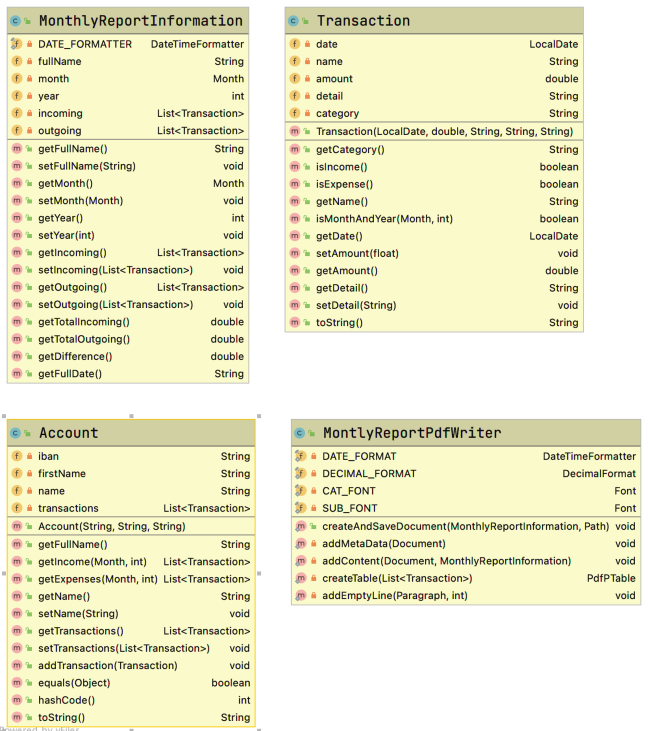
\includegraphics[width=\textwidth]{./images/chapter3/exercise-class-diagram} 

\end{oefening}

\begin{thebibliography}{9}
\bibitem{spring-web}
https://docs.spring.io/spring-framework/docs/current/reference/html/overview.html

\bibitem{lamport94}
Leslie Lamport (1994) \emph{\LaTeX: a document preparation system}, Addison
Wesley, Massachusetts, 2nd ed.


\end{thebibliography}